\chapter{Literature Review}\label{ch:literature-review}
There is a considerable amount of research in the area of resource allocation and task pricing in cloud computing,
where auction mechanisms are used to deal with competition.
Section~\ref{sec:resource-allocation-and-pricing-in-cloud-computing} presents the different approaches to resource
allocation and pricing mechanisms in Cloud Computing.

The proposed solution of the project (presented in chapter~\ref{ch:proposed-solution}) uses a form of
machine learning, called Reinforcement Learning to train agents. Section~\ref{sec:reinforcement-learning} covers the current
state-of-the-art algorithms in Q learning and policy gradient research.

\section{Resource allocation and pricing in Cloud Computing}\label{sec:resource-allocation-and-pricing-in-cloud-computing}
A majority of approaches taken for task pricing and resource allocation in Cloud Computing uses a fixed resource
allocation mechanism, such that each user requests a fixed amount of resources for a task from a server. However this
mechanism, as previously explained, provides no control for the server over the quantity of resource allocated to a task,
only determining the task's price. As a result, a majority of approaches don't consider the server's management of
resource allocation. Thus research has focused on designing efficient and strategyproof auction mechanisms.

Work by~\cite{KUMAR2017234} provides a systematic study of double auction mechanisms that are suitable for a range
of distributed systems like Grid computing, Cloud computing, Inter-Cloud systems. The work reviewed 21 different
proposed auction mechanisms over a range of important auction properties like Economic Efficiency,
Incentive Compatibility and Budget-Balance. In a majority of the proposed auction mechanisms, truthfulness was only
considered for the user, thus a Truthful Multi-Unit Double auction mechanism was presented as such that both users and
server should act truthfully.

Deep Reinforcement Learning was implemented by~\cite{Du2019} to learn resource placement and pricing in order to
maximise cloud profits. Deep neural network models with Long/Short Term Memory units enabled state-of-the-art online
cloud resource allocation and task pricing algorithms that had significantly better results than traditionally
online mechanisms with that profit made and number of users accepted. The system considered both the pricing and
placement of virtual machines in the system to maximise the profits of cloud providers through the use of Deep
Deterministic Policy Gradient~\citep{ddpg} to train agents. Users would request a type of virtual machine from the
system that a server would allocate to a user where the price and placement of the virtual machine with a known fixed
resource requirements where the price and server to be allocated to chosen by a neural network agents. The deep
Reinforcement Learning models were trained using real-world cloud workloads and achieved significantly high profit even
in worst-case scenarios.

Some approaches have been taken to increase flexibility within Fog Cloud Computing~\citep{Bi2019} through efficient
distribution of data centers and connections to maximise social welfare. A truthful online mechanism was
proposed that was incentive compatible and individually rational, to allow tasks to arrive over time by solving a
integer programming optimisation problem. Similar research in~\cite{vaji_infocom}, considers the placement of code/data
needed to run specific tasks over time where the demands change over time while also considering the operational costs
and system stability. An approximation algorithm achieved 90\% of the optimal social welfare by converting the problem
to a set function optimisation problem.

Previous work proposed the novel resource allocation mechanism and optimisation problem that this project works to
expand~\citep{FlexibleResourceAllocation}. The paper presents three mechanisms for the optimisation problem,
one to maximise the social welfare and two auction mechanisms for self-interested users. The Greedy algorithm presented
allows for quick approximation of a solution through the use of several heuristics in order to maximise the social
welfare. Results found that the algorithm achieved over 90\% of the optimal solution given certain heuristics compared
to a fixed resource allocation solution that achieved 70\%. The algorithm has polynomial time complexity with a lower
bound of $\frac{1}{n}$ however in practice achieves significantly better results. \\
The work also presented a novel decentralised iterative auction mechanism inspired by the VCG
mechanism~\citep{vickrey, Clarke, groves} in order to iteratively increase a task's price. As a result, a task doesn't
reveal its private task value that is believed to be particularly interest within military tactical network where countries
do not need to reveal the important of a task to another coalition country but allow them to run the task. The auction
mechanism achieves over 90\% of the optimal solution due to iteratively solving of a specialised server optimisation problem.
The third algorithm is an implementation of a single parameter auction~\citep{nisan2007algorithmic_critical_value} using
the greedy algorithm to find the critical value for each task. Using the greedy algorithm with a monotonic value density
function means the auction is incentive compatible and inherits the social welfare performance and polynomial time
complexity of the greedy mechanism.

\section{Reinforcement Learning}\label{sec:reinforcement-learning}
Computer scientists have always been interested in comparing computers against humans~\citep{turing1950computing} with a
key characteristic of humans is the ability to learn from experience. An ability Computers must have this programed in
and so researchers have invented a variety of ways for computers to do this. These are broadly
grouped into three categories: Supervised, Unsupervised and Reinforcement Learning. Supervised learning uses inputs
that are mapped to known outputs, an example is image classifications. Unsupervised learning in comparison doesn't have
a known output for a set of inputs, instead algorithms try to find links between similar data, for example data
clustering.

However both of these techniques are not applicable for cases where agents must interact with an environment making a
series of actions that result in rewards over time. Algorithms designed for these problems fall into the category of
Reinforcement Learning where agents select actions based on an environment state that generate the result state and
reward from the action as shown in figure~\ref{fig:reinforcement_learning}.

\begin{figure}[h]
    \centering
    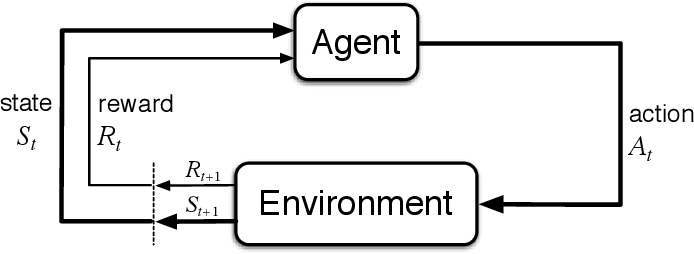
\includegraphics[width=10cm]{figures/1_background_lit_figs/agent_env_interaction.png}
    \caption{Reinforcement learning model (Source: ~\cite{Sutton1998})}
    \label{fig:reinforcement_learning}
\end{figure}

Q-learning~\citep{watkins1992q-learning} is a learning method used for estimating an action-value function,
called the Q value, that forms the basis of modern Reinforcement Learning algorithms. The Q value represents the
estimated discounted reward in the future given an action in a particular state. Equation~\eqref{eq:q_value} gives a
mathematically description where rewards in the future are discounted. A recursive version of this equation can be
formulated as equation~\eqref{eq:q_learning_recursive} where the next state is the max Q value of the next state-action.
Agents can be trained to approximate the Q value using equation~\eqref{eq:q_learning} through the used of a table
of state action pairs.

\begin{align}
    Q(s_t, a_t) = E[R_{t+1} + \gamma R_{t+2} + \gamma^2 R_{t+2} + \cdots ] \label{eq:q_value} \\
    Q(s_t, a_t) = r_t + \gamma \text{max}_a Q(s_{t+1} , a) \label{eq:q_learning_recursive} \\
    Q(s_t, a_t) = Q(s_t, a_t) + \alpha \cdot (r_t + \gamma \cdot \text{max}_a Q(s_{t+1} , a) - Q(s_t, a_t) ) \label{eq:q_learning}
\end{align}

However the curse of dimensionally was found to be a major problem for using Q learning as the number of states
or actions increased, the table grows exponentially in length as well. This made the method impractical for problems
with large state spaces due to both the table size and the required training time for agents.

Therefore function approximators are used to circumvent this problem, typically done using neural networks due to their
ability to approximate any function~\citep{csaji2001approximation} and to be trained using gradient descent.
Work by~\cite{atari}, implemented a deep Q network (DQN) to achieve state-of-the-art performance in six
of seven games tested as part of the Atari game engine, with three of these scores being superhuman. This was done
through using of two different neural network, a model and target network in which the target network is slowly
updated by the model network to act as a slowly updating target Q value. An experience replay buffer was also
implemented to enable the agent to learn from previous actions. \\
Follow up work by~\cite{mnih2015humanlevel} found that with no modifications to the hyperparameters, neural network or
training method; state-of-the-art results were achieved in almost all 49 Atari games with superhuman results in 29 of
these games. The work showed that deep neural networks could be trained through observing just the raw game pixels and
of the game score over time to achieve scores better than those humanly possibly.

Due to this research, a large number of heuristics have been proposed to the loss function~\citep{doubledqn},
network architecture~\citep{duelingdqn}, experience replay buffer~\citep{prioritizedexperiencereplay} and more to
improve the algorithm. A combined agent~\citep{rainbow} applying a range of heuristics enabling it to
achieved over 200\% of the original DQN algorithm in score.

\begin{wrapfigure}{l}{0.5\textwidth}
    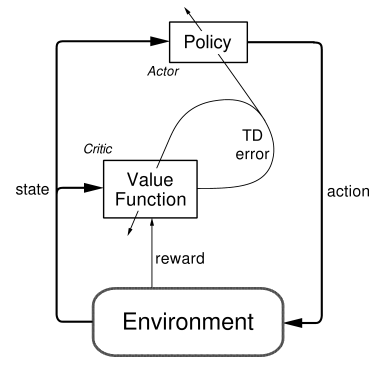
\includegraphics[width=0.5\textwidth]{figures/2_background_lit_figs/actor-critic.png}
    \caption{Actor Critic model (Source: ~\cite{Sutton1998})}
    \label{fig:actor-critic-model}
\end{wrapfigure}

Policy gradient agents, shown in figure~\ref{fig:actor-critic-model}, using the base of Q-learning separate the action
selection policy from the Q-value function known as the critic. In deep Q networks, actions are selected on the maximum
Q-value for all of the actions, however this requires actions to be discretized. By splitting the actions from the Q
values, an actor chooses an action based on the environment state allowing for both discrete and continuous action space
to be utilised. The critic network is trained almost identically to the DQN agent except fro the use of a soft target update.
While the actor network is trained through gradient ascent and the critic evaluation to increase the value. This has the
advantage of the action policy being trained directly compare to DQN agents where used an epsilon greedy action selection
policy however agents can also get stuck in local maxima's. As a result policy gradient has been
used to master the game of Go~\citep{silver2017mastering} and achieve top 1\% in both
Dota 2~\citep{OpenAI_dota} and Starcraft 2~\citep{starcraft2} video games.